%% Support sites:
%% http://www.michaelshell.org/tex/ieeetran/
%% http://www.ctan.org/tex-archive/macros/latex/contrib/IEEEtran/
%% http://www.ieee.org/

% The testflow support page is at:
% http://www.michaelshell.org/tex/testflow/

\documentclass[journal,12pt]{IEEEtran}

%\usepackage{blindtext}
\usepackage{graphicx}
\usepackage{cite}
\usepackage{float}
\usepackage[usenames,dvipsnames]{color}
\usepackage[english]{babel}
\usepackage{csquotes}

\definecolor{blue}{cmyk}{1.0,0.1,0.0,0.0}
\definecolor{orange}{cmyk}{0.0,0.45,1.0,0.0}
\definecolor{red}{cmyk}{0.0,1.0,0.5,0.0}
\definecolor{green}{cmyk}{0.7,0.0,1.0,0.0}
% correct bad hyphenation here
\hyphenation{op-tical net-works semi-conduc-tor}

%\renewenvironment{titlepage}
%{}

\title{Do No Harm: Are Rainbow Colormaps Dangerous? \\}
\author{Derek~Miller \\ Brigham Young University}% <-this % stops a space


\begin{document}

% make the title area
\begin{titlepage}
\maketitle
\thispagestyle{empty}
%\vspace*{\fill}

\begin{abstract}
Controversies and contradictions
surround the choice of colormaps in data visualization.
Colormaps are used to display complex data sets by
representing data points as colors on a continuous color scale. The scientific
community is divided on whether rainbow colormaps
adequately represent data in colored visualizations. Some point to evidence in medical imaging
that suggests the rainbow colormap distorts data, resulting in slower and 
less accurate data interpretation. Others have shown that the
scientific community is used to reading graphics with rainbow
color schemes and are no less accurate than others who use
a different color scheme. This document compares rainbow colormaps
to perceptually uniform colormaps.
To avoid errors in data interpretation, some scientific software programs
have changed their default colormap away from the rainbow scheme.
Nevertheless, the rainbow colormap
continues to be used in scientific literature.
\end{abstract}
\tableofcontents
\vspace*{\fill}
\end{titlepage}

\IEEEpeerreviewmaketitle

\section{Introduction}

Scientific progress depends on the ability to interpret data correctly. Rigorous data analysis
using scientific computing software is often desirable, but this takes time and concentration.
In many applications of science, it is simply impractical to perform lengthy analyses for every
experiment. Visual representations of data
allow scientists to interpret data quickly.
For example, a radiologist can determine the
type and severity of a bone fracture by looking at an
image representation of X-ray data. This allows her to make decisions on what treatments will be most effective
for the fracture. While most bone fractures are easy to see using X-ray technology, some data insights are
harder to find. Visualizations of complex data sets use color to highlight important features
in the data by turning numbers into colors. Scientists agree that the use of color is desirable in many applications.
However, many disagree over how color should be used when representing data.

One of the dominant controversies in scientific visualization involves the use of colormaps.
A colormap is a function that assigns data points to
an ordering of colors. Nathaniel Smith
calls them ``an interface between the data and your
brain \cite{viridis}'' since they allow the user to interact with data in a visual form.
When judiciously chosen, colormaps reveal hidden structure that would go unnoticed
otherwise. On the other hand, a careless colormap selection may distort the data,
leading viewers to false insights. This has
serious consequences, especially in medicine and public health \cite{arteryvis,choropleth}.
Doctors rely on visualization software to interpret medical
data correctly and properly diagnose and treat disease.
Citizens and politicians vote on public health policy based on data presented 
in visual form. These scientific disciplines have developed standards that determine
how to perform rigorous, consistent, and reproducible data analysis. However,
there is debate among scientists about colormap standards in data visualization---or
whether there should be colormap standards at all.

Of all the colormaps available, none draws more criticism and debate than colormaps that use a rainbow
color scheme. Readers of scientific literature will recognize the rainbow colormap. 
It appears often in scientific publications and has 
broad appeal in the scientific community
\cite{endofrainbow, rainbowstill, spectralschemes,choropleth}.
Despite its prevalence, 
many scientists oppose rainbow-gradient representations of data
\cite{rainbowstill, endofrainbow, viridis,arteryvis}.
In one study, medical students were
asked to identify risk factors for heart disease in visualizations
of artery data. On average, the participants
using rainbow-colored visualizations took more time
and made more errors than participants using divergence-colored visualizations. 
Furthermore, the participants ``thought they did well using the rainbow color
map even when in reality they did not perform as well
as the participants who used the diverging color map
\cite{arteryvis}.'' This compelling evidence suggests
that the rainbow colormap is clearly inferior to other
colormaps.

Others disagree. They claim that users have learned to
read data with the rainbow colormap and prefer its
aesthetic appeal \cite{spectralschemes, choropleth}. One
experiment tested data interpretation accuracy under
diverging, sequential, and spectral (rainbow) color
schemes. ``Of 63 subjects who evaluated spectral and
sequential schemes, 56 percent selected spectral as the
best...We had expected the spectral scheme to interfere
with map-reading accuracy and with understanding
map patterns, but this did not occur,'' Brewer writes.
``Our subjects preferred the spectral scheme
and performed well with it \cite{spectralschemes}.''
While the rainbow colormap did not outperform other colormaps, it
appears to do no harm. Users can accurately interpret
rainbow-colored data visualizations.

This literature review explores the advantages and disadvantages
of rainbow colormaps, why they are preferred by some
scientists and discouraged by others, and how spectral color schemes are used
in applied data analysis. First, this review covers important aspects of color science
necessary for effective colormap creation. Then, it will
address perception issues that affect color interpretation. 
Finally, the rainbow colormap will be evaluated alongside a discussion of rainbow colormap applications
in medical imaging and cartography.

\section{Colormap Fundamentals}

Colormaps assign data points to colors. This seems straightforward, but color assignment
depends on sophisticated mathematics and research in human perception. 
Color is both a physical phenomenon and a perceptual illusion \cite{endofrainbow}.
When light reaches our eyes, photoreceptors called cones detect light at certain wavelengths.
The cones send signals to the brain, which interprets the information,
and generates the perception we call color \cite{viridis}. Humans sometimes perceive the same
colors differently. In fact, the question of whether two colors are the same has motivated
research in color theory for decades and continues to play a central role in colormap 
evaluation.

\subsection{Color Models and Spaces}

To avoid ambiguity when talking about color, scientists use
color models---abstract mathematical representations that
describe a color as a collection of numbers.
When a color model is used with a specific medium such as a digital screen or a printer, the resulting set
of colors is called a color space \cite{colorimetry}. For example, the RGB model
describes color as the combination of red, green, and
blue light. A computer screen renders color using the
RGB model. The color produced by digital screens
with the RGB model is a color space. Another important example is the
CMYK model, which describes color as combinations of
cyan, magenta, yellow, and black. Printers produce colors using this model
\cite{colormapping}. The different combinations of cyan, magenta, yellow, and black
ink used by a printer constitutes a color space.

Most color spaces produce a similar set of colors. However, some colors
do not translate well between color spaces. Consider the following list:
\begin{itemize}
\item \textcolor{blue}{\textbf{Blue}}
\item \textcolor{red}{\textbf{Red}}
\item \textcolor{green}{\textbf{Green}}
\item \textcolor{orange}{\textbf{Orange}}
\end{itemize}
When this document is viewed digitally, the colors look
different than the colors on a printed copy. This represents
a transformation from an RGB color space to a CMYK color space \cite{colorvblackwhite}.
Color may not appear the same when transformed from one color space to another.
This is problematic if color needs to be consistent across
different media when presenting data visualizations.
For these reasons, it is helpful to understand some history in color model development.

\subsection{Early Color Models}

Much of the early work in color theory was focused on describing light as a physical phenomenon.
The first of these was the trichromatic theory of color. 
Developed by Thomas Young in 1802 and extended quantitatively by 
Hermann von Helmholtz in 1894, the theory revealed that photoreceptors
in the retina of the eye responded to long, medium, and short wavelengths of light, 
roughly corresponding to red, green, and blue color \cite{colorimetry}.
Shortly after, a breakthrough in color perception came when
Albert Munsell developed the Munsell Color Specification System in the early twentieth century.
It was developed by testing the appearance of colored paint chips on a variety of individuals.
The results revealed that color appearance is made up of
three independent variables---hue, chroma, and lightness.
This development led to the more
widely known HSL model which describes the perceptual attributes of color as combinations of hue,
saturation, and lightness\cite{colormapping,colorimetry}.
``This system
divides up the colors humans are capable of perceiving
into equal perceptual divisions of color lightness and
color saturation for each color hue. \cite{colormapping}''
Hue refers to the attribute generally associated with the color name (i.e. red,
orange, yellow, green, blue). Saturation is the intensity of the hue. In
physical terms, it is the purity of the light wave frequency. Lightness is the
amount of light emitted by a color \cite{colorguidelines}. Low lightness results in a darker color;
high lightness results in a lighter color.

The Munsell color system was a good way to describe the appearance of color but it did
not prescribe a way to create the same colors consistently.
This required more precise color models. In the early twentieth century,
The Commision Internationale de l'Eclairage (CIE) began developing robust color models
that allowed for color consistency. It was CIE who first developed the first reliable
RBG color model \cite{colorimetry}.
After the RGB model, CIE developed the CIEXYZ model in 1931
which became widely accepted. It is still used today and is critical to colormap creation
and evalutation. Many colormaps use models built with CIEXYZ as their foundation \cite{viridis}.
This model is particularly important because it has an objective scientific interpretation.
Its development focused on testing measurable, physical properties of light
against human color perception by way of color matching experiments 
\cite{colorimetry}. The results found that some colors look identical despite having very different physical
properties. This model specifies which wavelengths of light humans 
are capable of seeing. This set of wavelengths is known as the visible electromagnetic
spectrum and is the physical description of the rainbow \cite{colormapping}. This is the model
that describes a rainbow colormap.

\subsection{Perceptually Uniform Models}

The CIEXYZ color model transformed color science. Colors could now be precisely defined and replicated.
Using this technology, scientists were able to be more precise with color experiments.
They discovered that while CIEXYZ is a good descriptive model of color from a physical standpoint, it
is not a model of perceptual color distance \cite{viridis}.
To better understand the
perceptual difference between colors, CIE set out to
transform the CIEXYZ model into a perceptually uniform color model.

A sequence of colors where each color seems equally different from its neighbors
would be called a perceptually uniform color sequence. Perceptual uniformity means that
``equal steps in the data variable will be perceived as equal steps in the representation \cite{endofrainbow}.''
In 1976, CIE produced two perceptually uniform color models, CIELUV and CIELAB \cite{colorimetry}.
These are both commonly used as reliable models of color distance. Some have used these models
to create perceptually uniform colormaps \cite{viridis,matlab}.
After adjusting some deficiencies, CIE
released new perceptually uniform color models in 2002. These models are collectively known as 
the CIECAM02 color model family. In particular, CIE recommends using CIECAM02-UCS as the best
performing model of color distance \cite{ciecam02}.
One of the primary differences between CIELAB and CIECAM02-UCS is that the latter
is more perceptually uniform between similar colors than distant colors \cite{ciecam02}.
Because of this, some have argued that
perceptually uniform colormaps will be best when created using the CIECAM02-UCS model \cite{viridis}.
While CIECAM02-UCS is the best perceptually uniform model to date, the differences between competing models are subtle.

The other motivation for developing perceptually
uniform color models is to produce consistent colors across different media.
These models do not preserve absolute color, but perceived color difference tends
to remain the same across all media \cite{ciecam02}.
This reduces color conversion problems when the color model changes.

\section{Color Perception}

The previous section discussed attempts to quantify the effects of color.
This section addresses psychological aspects of color through color schemes,
simultaneous contrast, and color deficiency.

\subsection{Color Schemes}

\begin{figure}
\centering
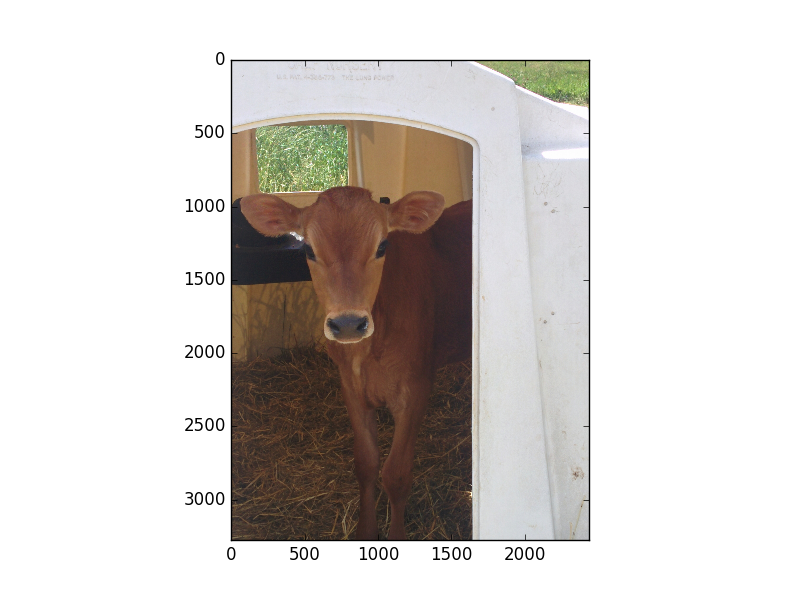
\includegraphics[width=2in]{calf_original} \\
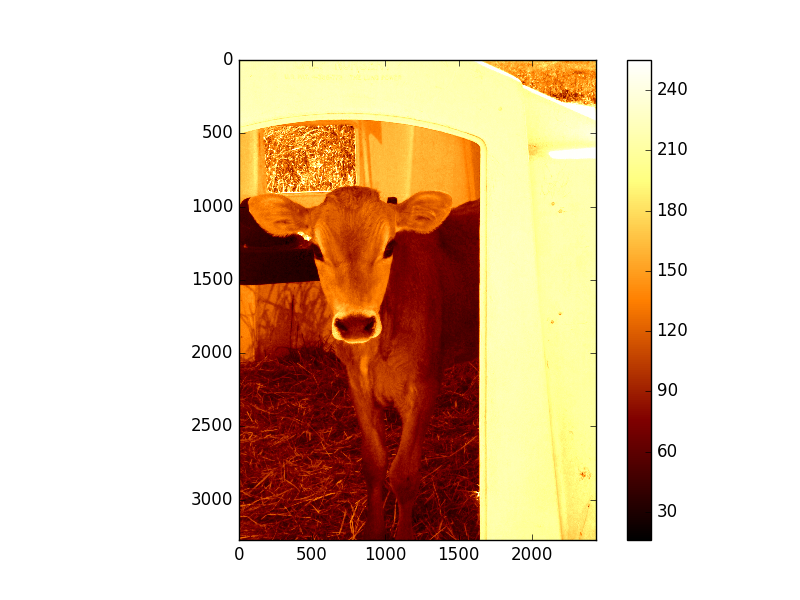
\includegraphics[width=2in]{calf_sequential} \\
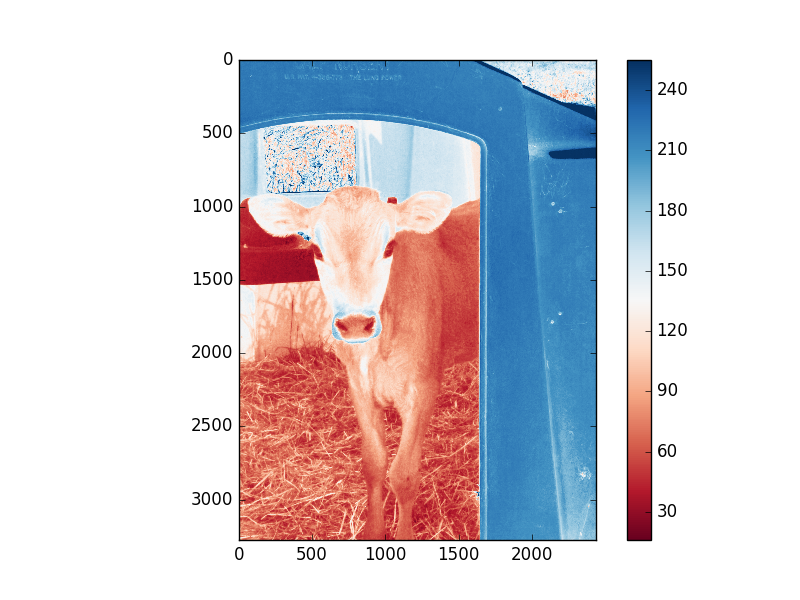
\includegraphics[width=2in]{calf_diverging} \\
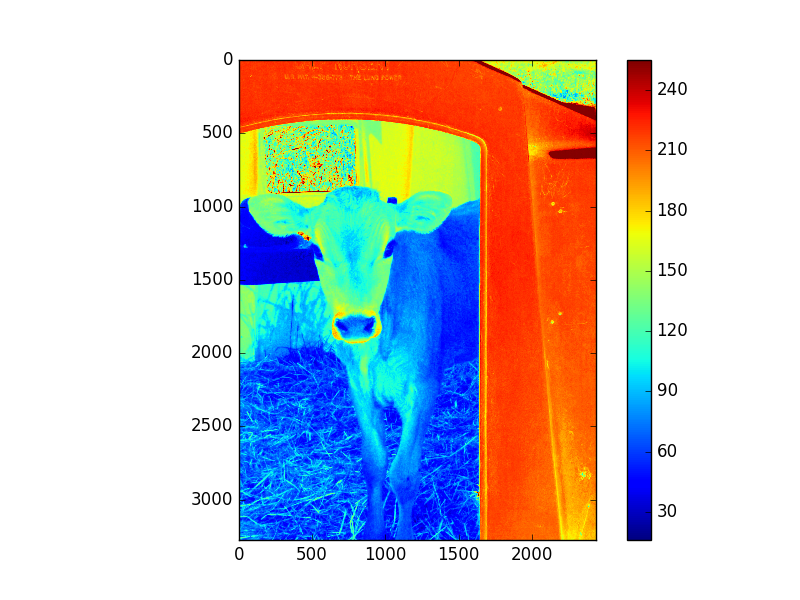
\includegraphics[width=2in]{calf_rainbow} \\
\caption{An image of a calf. The calf image plotted with a
sequential, diverging, and rainbow colormap. These images were created by the author.}
\end{figure}

The main problem
when designing a colormap is how to order colors
from least to greatest. Some suggest
ordering colors by light wavelength. 
This ordering produces the familiar rainbow spectrum
starting with red, then orange,
yellow, green, blue, and so forth \cite{colormapping}.
This was especially popular among physicists and rainbow colormaps soon became the default
in many scientific software applications \cite{rainbowstill,matlab}.
An alternative method of constructing a color ordering is to choose a color scheme that matches the data.

There are three main types of color schemes used to create a colormap.
Sequential color schemes vary in lightness but do not
vary in hue. This color scheme works best when visualizing linear data, such as the altitude over a region.
If two sequential color schemes have different hues and are
connected at their lightest ends, it is called a diverging color scheme. This works best when
the data varies between two opposing values, as in the political leaning of each state plotted 
with red and blue. Qualitative color
schemes vary in hues with little variation in lightness
and saturation \cite{colormapping}. The rainbow colormap uses a continuous,
qualitative color scheme. This is also known as a spectral scheme \cite{spectralschemes}
See Fig. 1 for examples of image data plotted with 
sequential, diverging, and rainbow colormaps.

\subsection{Simultaneous Contrast}

When colors are placed near each other, it changes the way our eyes see that color,
a phenomenon called simultaneous contrast.
This makes colors appear more bright under diffused light
and competing bright colors lose their perceived brightness.

\begin{figure}
\centering
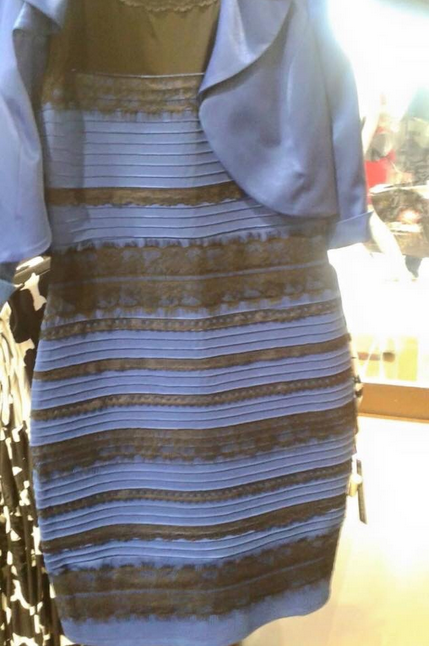
\includegraphics[width=2in]{colordress.png}%
\caption{An example of simultaneous contrast. Is the dress black-and-blue or white-and-gold?}
\end{figure}

An example of simultaneous contrast is the 
color-of-the-dress meme that became popular in 2015 \cite{colorofthedress}. A picture of a dress
(shown in Figure 2)
circulated on social media sites asking whether the dress was black-and-blue
or white-and-gold. This effect happens because our eyes perform a kind 
of normalization under different light conditions and alters
the perception of what the colors look like \cite{viridis}.
The same shade of gray can appear very different as the surrounding color changes.
Even though the colors are the same, they appear to be 
different because of the context that they are in. This means that sometimes
our eyes may detect color differences even when there are none.
Other times, color differences can't be detected easily or at all.
Colormaps with several highly saturated colors are particularly prone to the effects
of simultaneous contrast. If care is taken when looking at a visualization,
most people can correct for this issue.
However, this is more difficult for people who are color deficient.

\subsection{Color Deficiency}

Color deficiency, better known as colorblindness, results in colors falling on confusion lines---lines in which it
is difficult or impossible to distinguish between two colors in a color perception model \cite{colormapping}.
Color deficient viewers do not see the normal range of colors as their peers.
Full color deficiency results in black-and-white vision and is very rare.
The most common form of color deficiency results in confusing shades of red and green \cite{colorchoice}.
It seems reasonable to design data
visualizations with colorblindness in mind.
The estimated colorblind population is somewhere around 5-8\%
 \cite{colormapping,mapcvi,rainbowstill,spectralschemes,colorvblackwhite,matlab}.
For color deficient viewers reading a rainbow-colored data graphic,
high numeric values are displayed in reds and
the variation in green is not easy to interpret \cite{mapcvi}. The red and green
combination creates unnecessary confusion.

To correct for their deficiency, colorblind viewers use context
clues to distinguish between colors that easily confuse them.
Brewer has conducted extensive research into how color deficient
viewers interpret color-encoded information. She suggested several ways in which 
maps and information visualizations can be designed to be more colorblind friendly.
A common finding in her research, as well as others, is that colormaps are greatly
improved when the dark-to-light variation is controlled and used to show progression \cite{mapcvi}.
When converted to black and white, the visuals still preserve the nature of the data and are easy to interpret.
Caution is needed, however, when color encodings are converted to
grayscale. Some grayscale conversion algorithms alter the perception of the data \cite{colorvblackwhite}.
Still, the medical community seems to prefer grayscale representations as it is ``cautious about adding color
to its visualizations \cite{endofrainbow}''. The ability to distinguish between different values of lightness is
far easier than detecting differences in hue and saturation.

\begin{figure}
\centering
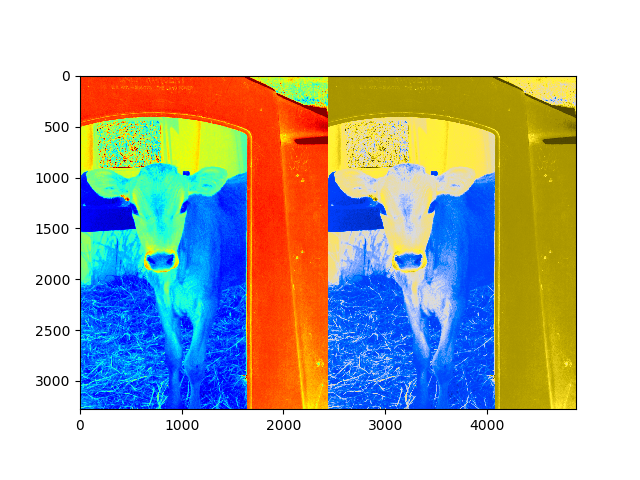
\includegraphics[width=2in]{colorblind_rainbow1.png}%
\caption{The rainbow colormaped image (left) and a colorblind approximation of the same image (right).}
\end{figure}

\section{Case Studies and Discussion}

The controversy surrounding the rainbow colormap does not appear to be random.
Certain industries disagree on how much the rainbow colormap should be 
discouraged. There is general agreement that rainbow colormaps are not as 
precise as perceptually uniform colormaps in representing data 
\cite{colorvblackwhite}. However, this 
does not mean that rainbow colormaps are discouraged in all cases
 \cite{spectralschemes}. 
Among the many uses of the rainbow colormap in the
literature, the two most cited are
medical imaging and cartography. Both care deeply about the use of color in 
their respective fields \cite{colorguidelines, standardmedimg}. Even within
 these applications, the recommended use of the rainbow colormap differs
 depending on the context.
 
\subsection{Cartography}

Maps are used to show public health information, the spread of disease, weather
forecasts, and other demographic data. This information is important to
 public policy and public awareness and is frequently shown
 using colored visualizations. Choosing an appropriate color scheme is not a trivial task. In her
article \textit{Mapping Mortality: Evaluating Color Schemes for Choropleth
Maps}, Cynthia Brewer shows that a judicious choice of color is ``worth 
the extra effort and expense'' because ``it permits greater accuracy in map
reading \cite{choropleth}.'' For public understanding of data, the rainbow colormap
seems to do no harm and users tend to prefer it.

Rainbows are not always good for maps, however. An assortment of colormaps were
developed and shown to be superior to rainbow schemes when used for oceaonography.
Sea level is an important metric in these contexts and a rainbow colormap poorly 
represents the coastline where land and sea meet. In this context, customized colormaps
outperform most other colormaps \cite{oceanography}. If the scientist knows that the data are in a particular form,
a customized colormap gives the best results.

\subsection{Medical Imaging}

The consequences for color misuse in medical imaging are severe. Research
already shows that the potential for diagnostic errors increases when 
rainbow color schemes are used \cite{arteryvis}. Color may not
be necessary and only used for convenience. However, some procedures (like virtual diagnosis) require 
medical images that must be interpreted using color \cite{standardmedimg}. In this case, it
is especially important that hardware components be standardized so that color
can be interpreted effectively. Since there are many manufacturers that produce
image processing software and display hardware, there is no consensus which 
color models or color mappings should be used by the medical community.
The Summit on Color in Medical Imaging
met to reach a consensus on how to standardize color use 
\cite{standardmedimg}. Images that are important to medicine but not exclusively
part of the community would not be held to these standards.

Bioinformatics and genetics are two fields related to medicine that 
could be exempt from the standards set in medical imaging. In fact, many tools
are being created now to analyze the vast amount of data that can be collected
in genetics. One such tool uses clustering techniques to find biomarkers in 
gene data. This software is written in MATLAB and designed to run on Microsoft
Windows and Linux x86 \cite{marvis}. This specific choice of software uses an
older vesion of MATLAB with a rainbow colormap as the default. 
Software updates and hardware limitations make it difficult to change 
the visualization system. This may be another reason why doctors prefer grayscale and
rainbow visualizations---it is too difficult to change.

\subsection{Evaluating Rainbow Colormaps}

What makes a colormap good?
One paper evaluated color schemes in terms of
three variables of the CIELUV color model. The first
is color distance. Since CIELUV is a model of color distance,
equally spaced colors on a colormap is considered desireable. The second variable is linear separation.
This refers to ``the ability to separate targets
from non-targets in the colour model being
used \cite{colorchoice}.'' If the
colors are not linearly separable, it
will be difficult to identify important insights in the data even though the
colors are mathematically different. The third variable
is color category, which refers to color regions where
there are both target and non-target elements \cite{colorchoice}.
These characteristics do not account for multidimensional data projected into two-dimensional
space. CheckViz attempts to account for this problem
by using a perceptually uniform color coding so that
distortions such as those described above are accounted for when 
scientists want multidimensional visualizations \cite{checkviz}.
However, the most practical way to evaluate a colormap is to consider whether the color
model, color space, and color scheme reflect the nature of the data being visualized.

Rainbow colormaps use a qualitative, spectral color scheme and appear to be defined
in terms of the CIEXYZ color model. They are not perceptually uniform because
the variation in lightness is inconsistent.
This has not stopped some from attempting to modify---and therefore preserve---the
rainbow colormap.
Sisneros et al created a colormap modification framework that smooths the variation
in luminance (or lightness) and chromaticity, which is a combination of saturation
and hue. Their method can be applied to any colormap to make it perceptually uniform.
However, they focused their efforts on improving the rainbow colormap, since it is still widely
used in science \cite{chasingrainbows}. Their improved rainbow colormap contains subdued colors that better
represent image data. 

The advantage of using rainbow colormaps is that users tend to prefer it
over other colormaps \cite{spectralschemes, choropleth, endofrainbow}. 
Depending on the data being visualized, the variety in hue can show relationships better than
a sequential, single-hue colormap. The rainbow colormap also has a long
history of use in scientific publications and many are already used
to reading data from this colormap. In her research involving map reading and color deficiency,
Cynthia Brewer found some surprising results. Colorblind viewers had slower reaction times than 
full color vision viewers
when working with maps that were supposedly colorblind-friendly.
Referring to a conversation
with a red-green color impaired individual, Brewer explains,
\begin{displayquote}
``Shown a map on which several categories of values were represented by the very same color,
this person was convinced that they were differentiable colors (to those with normal vision) that 
he could not distinguish. It was not until he was told that the colors really were identical
...that he discontinued his efforts to detect some difference between them. In other words,
he had learned not to trust what he saw; there must be a difference, and if he looked long enough
perhaps he could detect it. It is quite possible that, in general, those with color vision impairments
have become so accustomed to having difficulty with colors that they do not trust their first impressions, and
they take longer in color discrimination tasks than do people with normal color vision \cite{mapcvi}.''
\end{displayquote}
This is a strong argument for keeping rainbow colormaps if users have learned how to read them,
even if they are colorblind.

Some problems still need resolution, however.
A human interpreter might see artifacts in the data---areas where it looks like
something is there that doesn't actually exist. These false positives
 occur more often when the data lie in certain regions (as in
between blue, green, and yellow) \cite{colorchoice, endofrainbow,oceanography}.
It is still uncertain whether or not rainbow colormaps do harm, but most agree
that there are better alternatives that can be used instead.

Many recognize that choosing standards is difficult---especially about color \cite{standardmedimg}. 
Some recommend changing 
colormap defaults instead of setting standards \cite{viridis,matlab}. That way, some 
consistency can be maintained while still allowing variation in color choice.
This is the conclusion of visualization studies like the one 
carried out in the development of the HemoVis medical imaging program 
\cite{arteryvis}. It is not feasible to standardize visualization
software across all platforms and technologies.

\section{Conclusion}

Color is an essential attribute of data visualizations. Representing data
with color is best done through a colormap designed specifically for the data set to be visualized.
To be thoroughly constructed and evaluated, colormaps require a vast amount of knowledge.
Data visualization is important to many disciplines and involves subjects
as different as engineering, computer science, graphic design,
and psychology \cite{choropleth}. The recent development in color rendering technology has made it 
possible to develop and test many different colormaps. In particular, it seems clear that
the rainbow colormap has many undesirable properties for data representation.
It takes more time for viewers to interpret data with this colormap and they tend to
make mistakes when the data fall in areas where the color changes do not match 
equivalent changes in the data. There does not seem to be a problem in cartography
and people tend to prefer the rainbow colormap because it is familiar and aesthetically pleasing.
The extent to which these faults cause damage is unclear. However, it is reasonable to conclude
that other colormaps are superior to rainbow colormaps for most data sets.
This is the motivation for changing default colormaps to be perceptually uniform
in scientific software, as in Matplotlib's \textit{viridis} and MATLAB's \textit{perula} \cite{viridis,matlab}.
These alternatives are perceptually uniform and tend to represent generic data better.
The variety of colors is diminished and the darkness-to-lightness progression
is more consistent with human perception of color change.
There has been little to no research on the effects of using these new colormaps.

Perceptually uniform colormaps are more friendly to color
impaired individuals. When colors cannot be changed
to accomodate for color impairment, redundancy can be added to the visualization
so as to encode the same information the color represents as a small icon or by using
a different visual variable such as position or size. In contexts where data
interpretation needs to be precise and time-efficient, rainbow colormaps should be discouraged.
In applications where user preferences are valued over representational accuracy,
the rainbow colormap is acceptable. Scientists should 
encourage the use of perceptually uniform colormaps as the default colormap choice and phase out the rainbow colormap
in scientific literature.

%\ifCLASSOPTIONcaptionsoff
%  \newpage
%\fi

\newpage

\bibliographystyle{ieeetr}
\bibliography{litreview}

\end{document}



